\documentclass[xcolor=dvipsnames]{beamer}

%%% Packages %%%
\usepackage{graphicx}
\usepackage[utf8]{inputenc}
\usepackage{subfig}
\usepackage{tikz}
\usepackage[absolute, overlay]{textpos}
\usepackage{soul}
\usepackage{booktabs}
\usepackage{multicol}
\usepackage{multimedia} % For movies
\usepackage{pgfplots} % For generating random numbers for tikz 

\usetikzlibrary{calc}

%%% Creating Tarleton Purple %%%
\definecolor{TarletonPurple}{RGB}{79, 45, 127}


%%% Beamer Theme %%%
\usetheme{Szeged}
\usecolortheme[named=TarletonPurple]{structure}


%%% Graphics Path %%%
\graphicspath{{./images}}

%%% Title Page Info %%%
\title{SYNC or Swim}
\subtitle{A Particle Model of the Interaction within Fish Schools}
\author{David Ebert and Mikaela Jordan}
\institute{Tarleton State University}
\date{March 31, 2017}

%%% Making Reference Environment For Tarleton Picture %%%
\newenvironment{reference}[2]{
\begin{textblock*}{\textwidth}(#1,#2)              
  \footnotesize\it\bgroup\color{red!50!black}}{\egroup\end{textblock*}}


\begin{document}
\makeatletter
\def\beamer@framenotesbegin{
\begin{reference}{1mm}{1mm}
\tikz\node[opacity=1.0]{
\includegraphics[scale=0.25]{images/Tarleton_State_University}};
\end{reference} 
}

\frame{\titlepage}

\begin{frame}
	\frametitle{Synchronization}
	The coordination of events to operate a system in unison.\\ 
	Some natural physical examples:
	\begin{itemize}
		\item Circadian Rhythms
		\item Round of Applause (WHAT?!?! - Let's try it!)
	\end{itemize}
\end{frame}

\begin{frame}{Human Swarming - Example}
\begin{center}
% The movie won't play in a normal .pdf viewer. Okular works.
\movie[width=10.5cm,height=7.0cm, poster, showcontrols]{}{human_swarm.ogv}
\end{center}
\end{frame}

\begin{frame}
	\frametitle{Coupling}	
	One object influencing another by providing feedback. \\
	Real life examples
	\begin{itemize}
		\item Animal Swarming
	\end{itemize}
	\begin{center}
	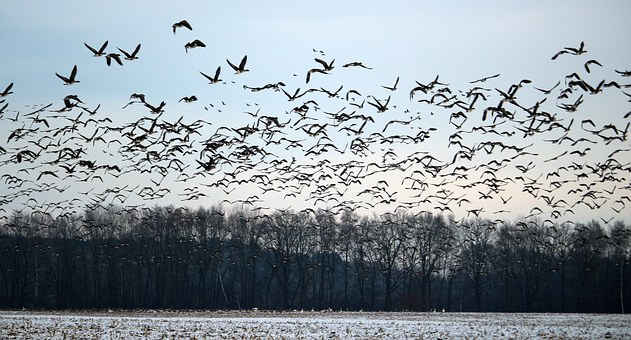
\includegraphics[scale=1.15]{images/geese_flock.jpg}
	\end{center}
\end{frame}

\begin{frame}
	\frametitle{Coupling}	
	One object influencing another by providing feedback. \\
	Real life examples
	\begin{itemize}
		\item Human Imitation (Memes/Trends)
	\end{itemize}
	\begin{center}
	
\includegraphics[scale=0.15]{images/salt_guy.jpg}
	\end{center}
\end{frame}

\begin{frame}
	\frametitle{Collective Behavior}
	\begin{center}
	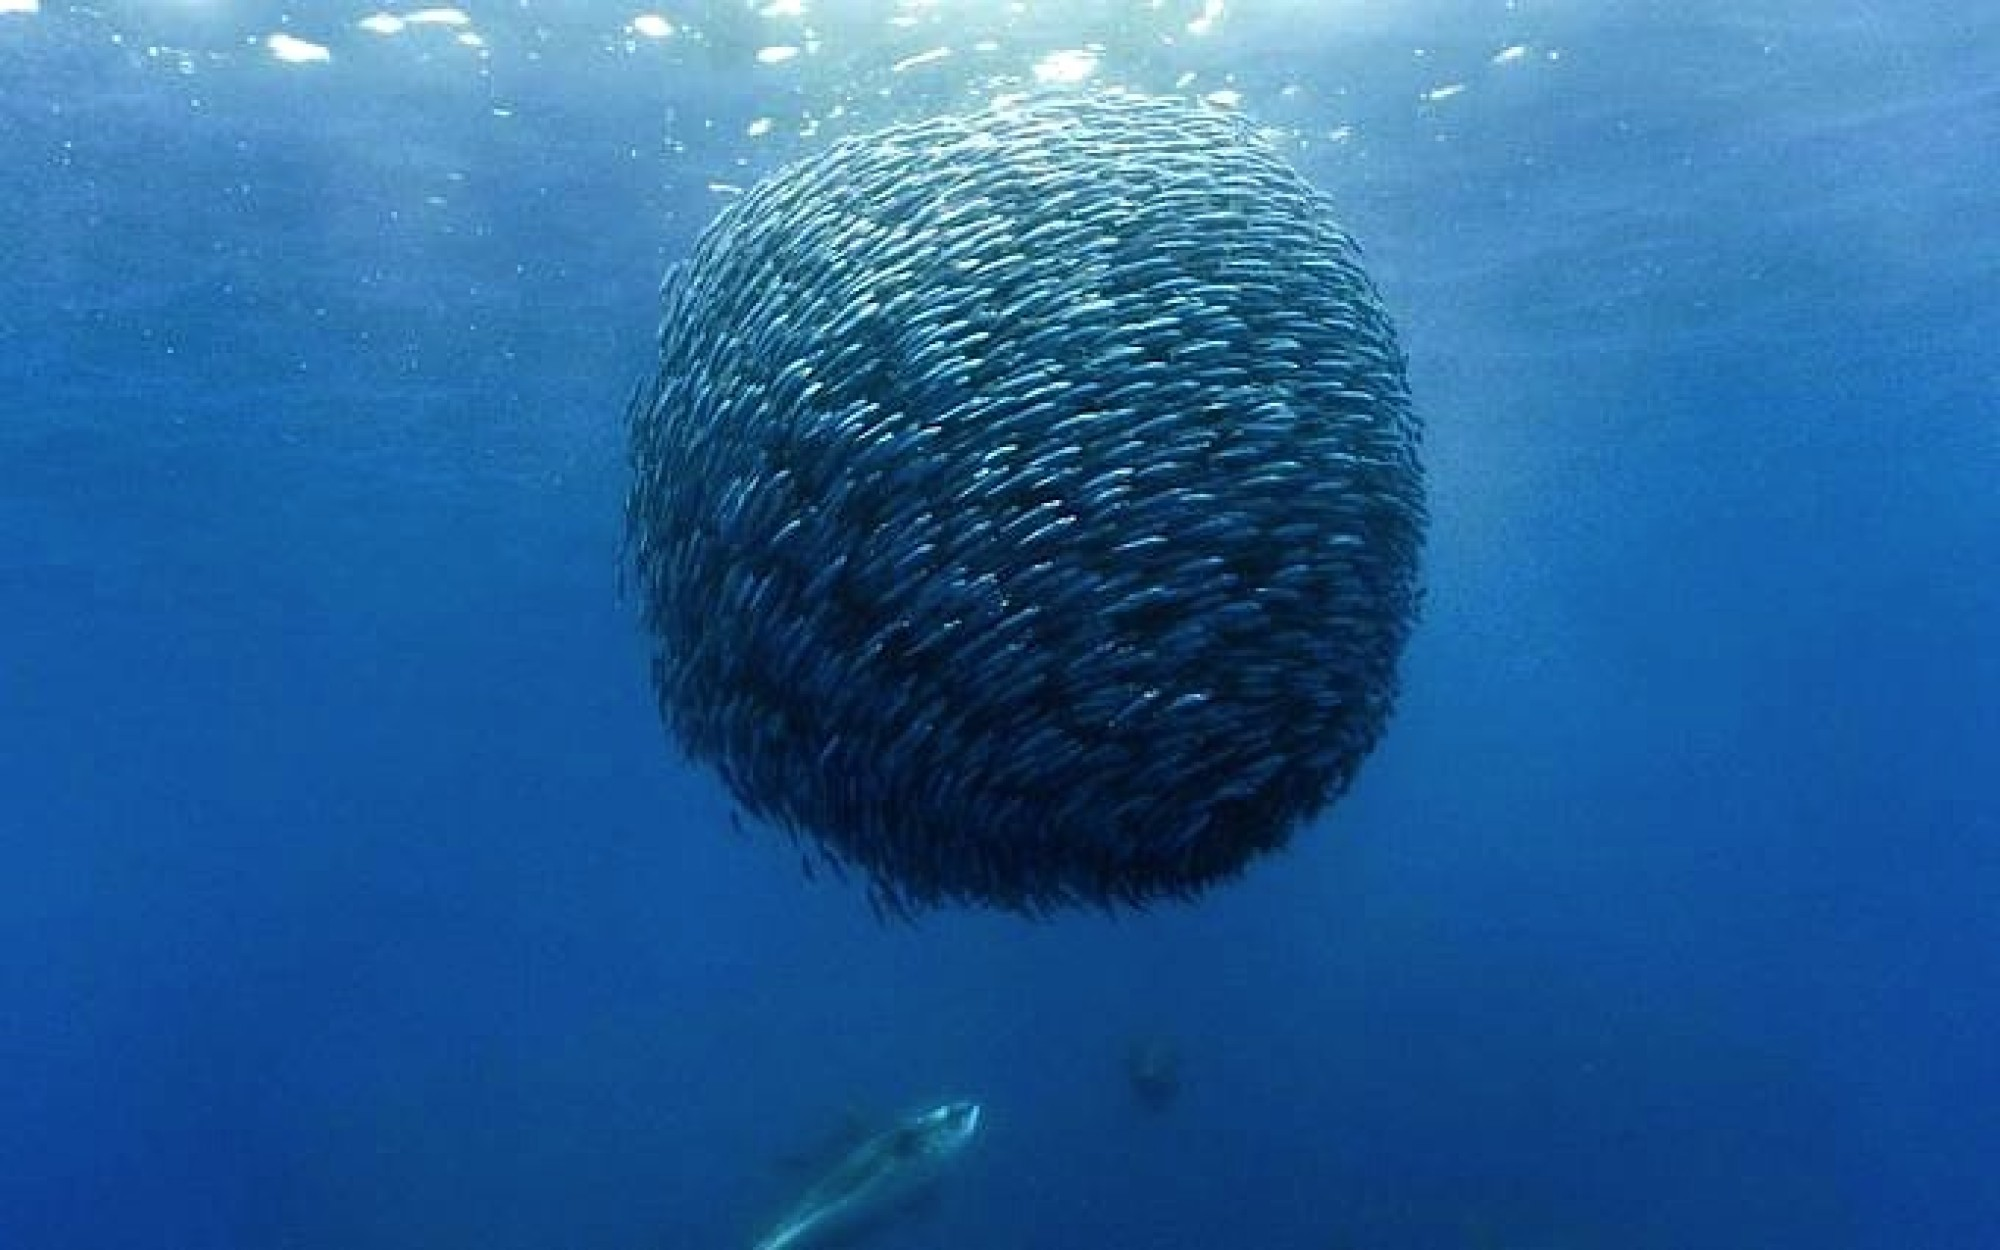
\includegraphics[scale=0.05]{images/fish_schoo.jpg}
	\end{center}
	\begin{itemize}
		\item The coordinated behavior of animals of the same species and the emergent properties that arise.
		\pause
		\item For mathematical purposes, consider a swarm as an emergent behavior with no central coordination that arises due to several simple instinctual rule that animals of a given species follow.
		\pause
		\item Other terms we will be using interchangeably with ``collective behavior'': swarm, school(specific to fish)
	\end{itemize}
\end{frame}

\begin{frame}
	\frametitle{Why Do We Care?}
	\begin{itemize}
			\item Learning C/CUDA
			\item Applying mathematical models to real life phenomenon
			\item How will environmental factors affect the animal aggregate
			\item How animal aggregates will affect the environment 
	\end{itemize}
\end{frame}

\begin{frame}
	\frametitle{The Basic Model}
	As a simple model/simulation of the swarm (schooling) behavior of fish, our model represents each fish adhering to the following three rules:
	\pause
	\begin{itemize}
		\item Move in the same direction as your neighbors
			\pause
		\item Remain close to neighbors
			\pause
		\item Avoid collisions with neighbors
	\end{itemize}
\end{frame}

\begin{frame}
	\frametitle{Coupling}
	Coupled oscillators are systems of masses connected by springs.
	\begin{center}
		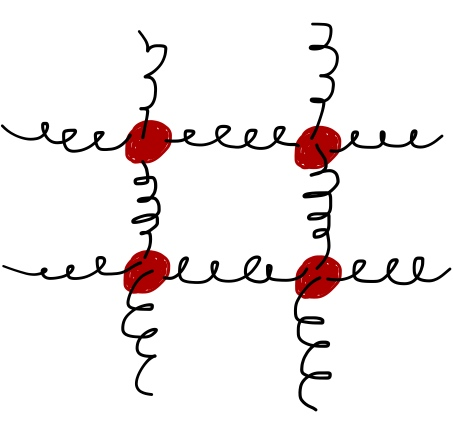
\includegraphics[scale=0.4]{images/coupled_oscillators}
	\end{center}
\end{frame}

\begin{frame}
	\frametitle{The Mathematics}
	\begin{itemize}
		\item Lagrangian Algorithm
		\begin{itemize}
			\item Agent Based Model following individual particles in school
		\end{itemize}
		\item Metric distance model - calculate forces on individual particles based on distance to other particles
	\end{itemize}
	\begin{figure}
		\centering
%		\begin{tikzpicture}[declare function={a(\x)=sqrt{\x^2 -1};},
%							declare function={b(\x)=-sqrt{\x^2 -1};},
%							declare function={c(\x)=sqrt{x^2 - 4};},
%							declare function={d(\x)=-sqrt{x^2 - 4};},
%							declare function={h(\x)=sqrt{x^2 - 6};},
%							declare function={f(\x)=-sqrt{x^2 - 6};}]
%			\draw[TarletonPurple, ultra thick] (0, 0) rectangle (10, 5);
%			\draw[TarletonPurple, ultra thick] (5, 5) -- (5, 0);
%			\foreach \x in {2.5, 7.5}{	
%				\fill[Emerald] (\x, 2.5) circle [radius=4pt];
%			}
%			\foreach \x [evaluate=\x as \xval using rand+2.5]in {1, ..., 3}{
%				\foreach \y [evaluate=\y as \yval using rand+2.5] in {1, ..., 2}{
%					\fill[Goldenrod] ($(\xval + 5, \yval)$) circle [radius=4pt];
%				}
%			}
%			\foreach \y [evaluate=\y as \yval using rnd*5] in {1, 2}{
%				\foreach \x [evaluate=\x as \xval using rnd+5.25] in {1, ..., 3}{
%					\fill[TarletonPurple] (\xval, \yval) circle [radius=4pt];
%				}
%			}
%%			\draw[TarletonPurple, ultra thick] (
%
%		\end{tikzpicture}

	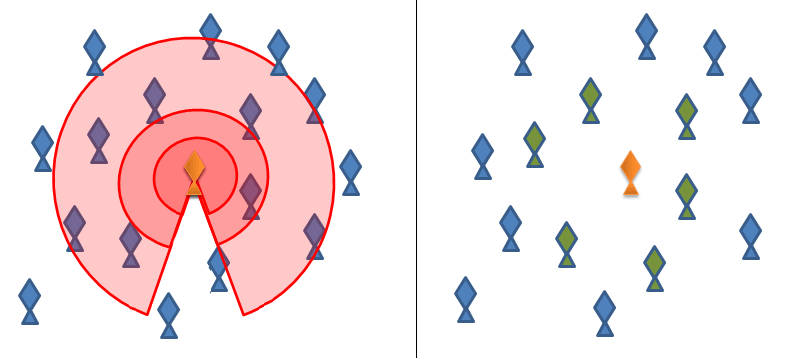
\includegraphics[scale=0.25]{images/distance_models.png}
	\end{figure}
\end{frame}

\begin{frame}
	\frametitle{Calculating Forces, Velocities, and Positions}
	At every timestep, the following calculations occur for each particle (let's call it particle $i$):
	\pause
	\begin{itemize}
		\item Calculate distance between particle $i$ and every other particle. \pause
		\item If the distance between some particle $j$ and particle $i$ is smaller than predefined search distance, then use Hooke's law to determine the forces between particle $j$ and particle $i$. \pause
		\item Use force calculated above to update particle $i$'s velocity as follows: \pause
			\begin{equation*}
				v_{i} = v_{i} + a_{i}dt
			\end{equation*} \pause
		\item And update particle $i$'s position using: \pause
			\begin{equation*}
				p_{i} = p_{i} + v_{i}dt	
			\end{equation*}

		
	\end{itemize}
\end{frame}

\begin{frame}
	\frametitle{Simulations}
\end{frame}

\begin{frame}
	\frametitle{Where Do We Go From Here?}
	\begin{itemize}
		\item Add initial conditions for species-specific parameters 
			\begin{itemize}
				\item Density of swarms, how they behave towards targets and obstacles, etc.
			\end{itemize}
		\item Move calculations from CPU to GPU to speed up calculation time
	\end{itemize}
\end{frame}

\begin{frame}
	\frametitle{References}
	\footnotesize{
	Barbaro, Alethea, Bjorn Birnir, and Kirk Taylor. \textit{Simulating the Collective} \\
	\hspace{0.5cm} \textit{Behavior of Schooling Fish With a Discrete Stochastic Model}. University\\
	\hspace{0.5cm} of Iceland. 2006. Web. \\
	
	\noindent Bernoff, Andrew J. ``Synchronization and Swarming: Clocks and Flocks.'' \\
	\hspace{0.5cm} Harvey Mudd College. \\
	
	\noindent Morale, Daniela, Vincenzo Capasso, and Karl Oelschlager.``An Interacting \\
	\hspace{0.5cm} Particle System Modelling Aggregation Behavior: From Individuals to\\
	\hspace{0.5cm} Populations''. \textit{Journal of Mathematical Biology}. 2004. Web.
	
	\noindent Parrish, Julia K., Steven V. Viscido, and Daniel Grunbaum. ``Self-Organized \\
	\hspace{0.5cm} Fish Schools: An Examination of Emergent Properties''. \\  
	\hspace{0.5cm} \textit{The Biological Bulletin} 202. 2002:296-305. Web. \\
	
	\noindent Schellinck, Jen, and Tony White. ``A Review of Attraction and Repulsion\\
	\hspace{0.5cm} Models of Aggregation: Methods, Findings, and a Discussion of Model \\
	\hspace{0.5cm} Validation''. \textit{Ecological Modelling} 222. 2011: 1897-1911. Web.
	}
\end{frame}

\begin{frame}
	\frametitle{THANK YOU} 
	Thank you to Dr. Wyatt and the Particle Modelling Lab for their time and resources.
	\begin{center}
		\Huge{QUESTIONS?}
	\end{center}
\end{frame}

\end{document}